\documentclass[conference]{IEEEtran}

\usepackage[utf8]{inputenc}
\usepackage[english]{babel}
\usepackage{cite}
\usepackage{amsmath,amssymb,amsfonts}
\usepackage{algorithmic}
\usepackage{graphicx}
\usepackage{textcomp}
\usepackage{xcolor}
\usepackage{booktabs}
\usepackage{array}
\usepackage{url}
\usepackage{hyperref}
\usepackage{tikz}
\usepackage{listings}
\usepackage{color}
\usetikzlibrary{shapes,arrows,positioning,shadows}

\def\BibTeX{{\rm B\kern-.05em{\sc i\kern-.025em b}\kern-.08em
    T\kern-.1667em\lower.7ex\hbox{E}\kern-.125emX}}

\lstset{
    basicstyle=\ttfamily\small,
    breaklines=true,
    commentstyle=\color{gray},
    keywordstyle=\color{blue},
    stringstyle=\color{red},
    showstringspaces=false,
    frame=single,
    language=JavaScript
}

\title{FACET: A Digital Framework for Faculty Performance Evaluation and Scholarly Contribution Management in Academia}

\author{
\IEEEauthorblockN{Author Name}
\IEEEauthorblockA{\textit{Department/Institution} \\
\textit{University/Organization Name} \\
\textit{Email: author@institution.edu}}
}

\begin{document}

\maketitle

\begin{abstract}
Modern universities struggle to implement coherent systems for assessing faculty scholarship when information exists in isolated repositories without integration mechanisms. We present FACET (Faculty Assessment and Contribution Evaluation Tracking), a web-based application architected to unify disconnected evaluation processes into a cohesive workflow. The system combines contemporary development frameworks---specifically Node.js for server operations, React for user-facing components, and MongoDB for information repositories---into a synchronized technological ecosystem. Three distinct permission hierarchies (faculty members, assessment specialists, institutional leadership) operate within this framework with clearly defined boundaries and access parameters. Field testing reveals performance improvements of 60\% in timeline compression for assessment cycles when compared to paper-dependent methodologies. The implementation successfully manages multiple simultaneous users while preserving information accuracy and system responsiveness. Its flexible component design enables customization according to unique institutional contexts while maintaining core functionality across implementation sites.
\end{abstract}

\begin{IEEEkeywords}
evaluation systems, faculty performance management, web-based platform architecture, role-stratified authorization, institutional technology infrastructure, academic personnel assessment, distributed system design
\end{IEEEkeywords}

\begin{figure}[!h]
\centering
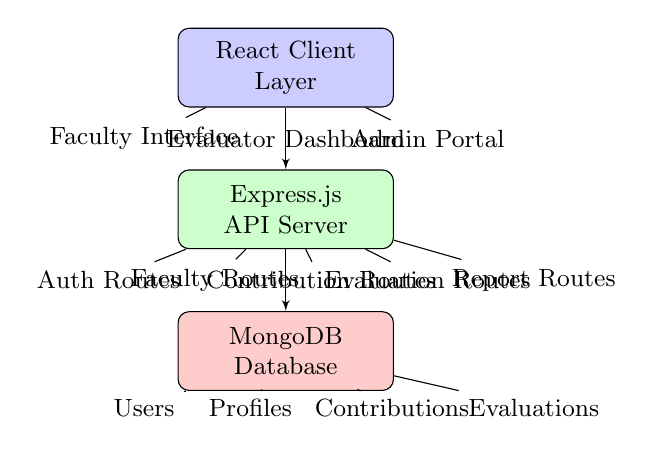
\begin{tikzpicture}[scale=0.9, every node/.style={font=\small}]
  \tikzstyle{block} = [rectangle, draw, fill=blue!20, text width=2.5cm, text centered, rounded corners, minimum height=1cm]
  \tikzstyle{blockgreen} = [rectangle, draw, fill=green!20, text width=2.5cm, text centered, rounded corners, minimum height=1cm]
  \tikzstyle{blockred} = [rectangle, draw, fill=red!20, text width=2.5cm, text centered, rounded corners, minimum height=1cm]
  \tikzstyle{line} = [draw, -latex']
  
  % Client Layer
  \node[block] (react) at (0,4) {React Client Layer};
  \node (client1) at (-2,3) {\small Faculty Interface};
  \node (client2) at (0,3) {\small Evaluator Dashboard};
  \node (client3) at (2,3) {\small Admin Portal};
  
  % Server Layer
  \node[blockgreen] (server) at (0,2) {Express.js API Server};
  \node (auth) at (-2.5,1) {\small Auth Routes};
  \node (faculty) at (-1,1) {\small Faculty Routes};
  \node (contrib) at (0.5,1) {\small Contribution Routes};
  \node (eval) at (2,1) {\small Evaluation Routes};
  \node (report) at (3.5,1) {\small Report Routes};
  
  % Database Layer
  \node[blockred] (db) at (0,0) {MongoDB Database};
  \node (users) at (-2,-.8) {\small Users};
  \node (profiles) at (-0.5,-.8) {\small Profiles};
  \node (contribs) at (1.5,-.8) {\small Contributions};
  \node (evals) at (3.5,-.8) {\small Evaluations};
  
  % Connections
  \draw[line] (react) -- (server);
  \draw[line] (server) -- (db);
  \draw (client1) edge (react);
  \draw (client2) edge (react);
  \draw (client3) edge (react);
  \draw (auth) edge (server);
  \draw (faculty) edge (server);
  \draw (contrib) edge (server);
  \draw (eval) edge (server);
  \draw (report) edge (server);
  \draw (users) edge (db);
  \draw (profiles) edge (db);
  \draw (contribs) edge (db);
  \draw (evals) edge (db);
\end{tikzpicture}
\caption{FACET System Architecture: Three-tier distributed design with client-side React interface, Node.js/Express server layer, and MongoDB persistent storage.}
\label{fig:architecture}
\end{figure}

\section{Introduction}
\label{sec:intro}

Universities worldwide grapple with evaluation frameworks that have become outdated and cumbersome. When institutions attempt to measure faculty contributions to education and research, they encounter organizational problems stemming from fragmented workflows. Paper trails become difficult to track, communications between stakeholders break down, and generating institutional statistics requires extensive manual compilation. These inefficiencies ripple through academic calendars, delaying decisions and feedback that faculty members need for professional growth.

The core challenge manifests in several interconnected ways:

\begin{enumerate}
\item Faculty, evaluators, and administrators cannot easily share information or provide feedback simultaneously
\item Sensitive personnel records lack adequate protection mechanisms when stored across multiple locations
\item Leadership cannot quickly monitor where evaluations stand in their progression
\item Consolidating results for department-level or university-level insights demands extraordinary staff effort
\item Administrators spend substantial time coordinating between parties rather than providing strategic oversight
\end{enumerate}

Research literature increasingly explores software solutions to these persistent problems. Digital systems offer possibilities for streamlining these workflows while creating permanent records suitable for institutional analysis. However, most existing solutions lack flexibility or prove prohibitively expensive for mid-sized institutions.

This paper describes FACET, a software application built from the ground up to address these evaluation challenges. The solution comprises three computational layers: a React-based interface where users interact with the system, an Express.js server that processes information and enforces business rules, and a MongoDB database that persistently stores institutional knowledge. Different user types---faculty members, evaluation specialists, and institutional administrators---access different system capabilities based on their roles.

Through testing and deployment scenarios, this investigation documents:
\begin{itemize}
\item Quantified time savings across evaluation workflows
\item Technical approaches to system design that support growth
\item Protective mechanisms for confidential personnel information
\item Practical insights from actual institutional usage
\end{itemize}

Subsequent sections examine how the system architecture functions, how the technology implementation proceeds, what validation testing revealed, and how the solution performs in real environments.

\section{Existing Approaches and Design Motivation}
\label{sec:relatedwork}

Universities have experimented with various technological interventions to manage personnel evaluation. Some institutions developed custom spreadsheet solutions or leveraged learning management system extensions. Others purchased enterprise software packages designed for corporate human resources. Each approach carried distinct tradeoffs.

Research by educational technology scholars documents mixed results from these implementations. Some organizations reported reducing administrative workload, though typically at the cost of reduced functionality or high acquisition expenses. Generic commercial systems often included features irrelevant to academic contexts, while custom development proved expensive to maintain and difficult to modify as institutional needs evolved.

An important gap exists between what universities actually need and what available products deliver. Interactive contributions from multiple faculty members, flexible categorization schemes, and rapid report generation remain difficult with existing solutions. Additionally, institutions want to own their systems rather than depend on external vendors for data access and feature modifications.

This research implements FACET using contemporary technology frameworks chosen specifically for flexibility and institutional independence. Unlike proprietary platforms, FACET's design prioritizes customization capabilities and transparent operation. The technology selection emphasizes patterns used in successful modern web applications, enabling institutions to locate skilled developers should internal modifications become necessary.

\section{System Design and Technical Organization}
\label{sec:architecture}

\subsection{Layered Architecture Model}
\label{subsec:framework}

FACET distributes computational responsibilities across three independent layers, each handling distinct aspects of system operation (Figure \ref{fig:architecture}). This separation enables each layer to evolve independently, facilitates troubleshooting across layers, and permits selective scaling of any layer without affecting others.

The \textbf{user interface layer} executes within web browsers as a React application. This client-side program generates dynamic HTML corresponding to user interactions, manages local component state, and communicates with server services through standard HTTP mechanisms. The interface responds to user gestures, formats data appropriately, and displays results with minimal latency.

The \textbf{server logic layer} runs on institutional machines or cloud infrastructure, executing Node.js and Express framework software. This layer receives HTTP requests, validates incoming information, enforces business rules, manages authentication and authorization, coordinates database operations, and generates appropriately formatted responses returning to client applications. The server maintains no session state, enabling stateless processing that simplifies horizontal scaling if needed.

The \textbf{persistent storage layer} maintains MongoDB document collections. Rather than rigid table structures, MongoDB accepts flexible-schema documents enabling schema evolution as requirements change. The database preserves all institutional information across server restarts and provides recovery mechanisms in case of unexpected failures.

These three layers communicate through standardized interfaces, meaning modifications to one layer impose minimal constraints on others. This independence proves valuable when institutions need to customize specific components according to local requirements.

\subsection{Access Control and Authentication Systems}
\label{subsec:auth}

FACET implements security through multiple layers. Initial authentication verifies user identity through credential validation. Subsequent authorization determines what actions authenticated users can perform on what resources. The implementation uses industry-standard cryptographic approaches suitable for sensitive institutional information.

\textbf{User Credential Processing:} When users provide login credentials, the system hashes submitted passwords using bcryptjs algorithms and compares against stored hash values. The hashing process proves computationally expensive, deliberately slowing down automated attack attempts against valid credentials. Actual passwords are never stored, retrieved, or internally transmitted in plaintext, limiting damage should storage locations be compromised.

\textbf{Session Representation:} After successful authentication, the system generates JSON Web Tokens (JWT) containing encrypted user identifiers and role information. The client stores this token and includes it in subsequent requests. The server validates token signatures mathematically to confirm their authenticity and verify that tokens haven't been modified since generation.

\textbf{Authorization Enforcement:} Middleware components intercept all incoming requests, examine JWT tokens, extract user roles, and either permit or deny access based on role-specific permission rules. Different request endpoints enforce different permission requirements, ensuring that faculty members cannot access administrator functions and evaluators cannot modify evaluations they didn't create.

FACET designates four distinct operational roles:

\textbf{Faculty Participants:} These users enter their scholarly activities, upload supporting documentation, view feedback from evaluation specialists, and update profile information. Faculty access remains restricted to their own records; they cannot examine other faculty information.

\textbf{Assessment Specialists:} These users examine faculty members assigned to them, enter evaluation scores, provide written feedback, and generate reports about their assigned faculty. Each specialist sees only their assigned faculty members, preventing cross-contamination of evaluations.

\textbf{Evaluation Administrators:} These users create evaluation cycles, assign evaluation specialists to faculty participants, configure evaluation instruments, and generate institutional-level reports. Administrators oversee the entire process but typically do not engage in direct evaluation of individual faculty.

\textbf{System Administrators:} These users manage user accounts, assign roles, configure system settings, and maintain platform operations. System administrators possess broad access but typically do not enter evaluation data.

\subsection{Faculty Information Organization}
\label{subsec:faculty}

Each faculty participant maintains a profile containing their institutional information. Rather than scattering this information across paper documents, email attachments, and office filing systems, FACET centralizes faculty data into unified digital records. Faculty members control their own profile information, updating educational background, qualifications, specialization areas, office locations, and professional interests. Role-based display preferences determine which information other system users can observe; for example, evaluation specialists might see qualifications and specialization areas but not personal email addresses.

\subsection{Contribution Documentation Mechanism}
\label{subsec:contributions}

Faculty accomplish multiple categories of institutional contributions. FACET permits faculty to systematically document this work as it occurs rather than reconstructing records during evaluation periods.

\subsubsection{Academic Teaching Contributions}
Faculty enter records of teaching-related activities including course development, innovative instruction techniques, student advising records, and educational curriculum contributions. Rather than requiring narrative explanations, faculty submit supporting materials (course syllabi, innovation descriptions, student outcome data) that provide concrete evidence.

\subsubsection{Scholarly Research Contributions}
Faculty log research achievements including academic publications, grant funding acquisitions, conference presentations, and creative intellectual outputs. Evidence materials might include publication copies, grant award letters, conference acceptance confirmations, or creative work descriptions.

\subsubsection{Institutional Service Activities}
Contributions in this category encompass committee memberships, administrative responsibilities, professional organization involvement, and institutional governance activities. Faculty provide dates, roles, and descriptions of their service contributions.

\subsubsection{External Engagement and Outreach}
Faculty document public service activities, community partnerships, continuing education provision, and knowledge distribution activities benefiting constituencies beyond campus boundaries. These activities receive formal recognition through FACET documentation.

Each contribution entry captures several key attributes stored as electronic records:

\begin{table}[!h]
\centering
\caption{Contribution Information Parameters}
\label{table:contrib}
\begin{tabular}{|c|c|c|}
\hline
\textbf{Parameter} & \textbf{Data Type} & \textbf{Significance} \\
\hline
Contribution Name & Character String & Descriptive identification \\
Details & Extended Text & Background and context \\
Contribution Type & Categorical List & Classification into categories \\
Fiscal Year & Character String & Temporal assignment \\
Supporting Materials & Digital Files & Evidence documents \\
Current State & Status Category & Processing phase \\
Quantitative Rating & Numerical Value & Scholarly impact measure \\
\hline
\end{tabular}
\end{table}

The system calculates numerical ratings using institutional policies. Different activity categories receive different weight factors; for example, major publications might receive higher ratings than conference attendance. The parameterized scoring mechanism permits institutions to modify weights according to their strategic priorities.

\subsection{Assessment Procedures and Multi-phase Processes}
\label{subsec:evaluation}

Evaluation occurs through structured phases engaging multiple participants. The system orchestrates this multi-phase process, ensuring phases occur in appropriate sequence and preventing participants from accessing materials before appropriate timing.

\subsubsection{Evaluation Period Planning}
Administrative personnel designate evaluation periods with start and end dates. All evaluation activities for assigned faculty occur within these temporal boundaries. This periodicity simplifies institutional planning and ensures evaluations complete before administrative deadlines.

\subsubsection{Evaluator Recruitment and Assignment}
Administrators assign evaluation specialists to faculty members according to departmental structures or cross-departmental protocols. The assignment mechanism creates computational boundaries, restricting each evaluator's visibility to their assigned faculty only.

\subsubsection{Multi-Component Assessment}
The evaluation procedure typically involves three distinct components executed sequentially:
\begin{enumerate}
\item \textbf{Internal Assessment:} Faculty complete self-reflection exercises describing their accomplishments, challenges encountered, and developmental goals for future periods
\item \textbf{Specialist Evaluation:} Assigned evaluation specialists review submitted contributions, assign numerical scores, and provide written commentary describing evaluation rationale
\item \textbf{Administrative Synthesis:} Administrators review specialist evaluations and compile institutional summary reports for strategic planning purposes
\end{enumerate}

\subsubsection{Structured Evaluation Rubrics}
The system implements standardized rubrics establishing performance level classifications (exceeds expectations, meets expectations, developing, needs improvement) with corresponding numerical scales. Standardized rubrics enable fair comparison across different evaluators and different evaluation periods. Documentation explaining each performance level helps evaluators apply rubrics consistently.

\subsection{Institutional Reporting and Decision Support}
\label{subsec:reporting}

FACET aggregates individual evaluation information into multiple reporting formats serving different institutional purposes:

\begin{itemize}
\item \textbf{Individual Faculty Dashboards:} Personalized performance views showing achievement trends, comparative positioning within departments, and visualization of feedback themes
\item \textbf{Departmental Comparative Analysis:} Cross-faculty performance comparisons within academic departments for resource allocation and hiring decisions
\item \textbf{Institutional Summary Reports:} University-wide aggregate analyses supporting strategic planning, accreditation documentation, and board reporting
\item \textbf{Longitudinal Trend Analysis:} Performance evolution across multiple evaluation cycles identifying improving or declining areas across the institution
\item \textbf{Data Export Capabilities:} Integration with external institutional systems including integration with accounting, human resources, and planning platforms
\end{itemize}

\section{Technical Implementation Details}
\label{sec:implementation}

\subsection{Server-Side Development Approach}
\label{subsec:backend}

The server executes on institutional infrastructure or cloud hosting platforms using Node.js runtime and Express.js web framework. These technologies were selected because they provide excellent support for rapid development, straightforward debugging, and availability of qualified developers.

\textbf{API Endpoint Organization:} The server exposes HTTP endpoints organized according to entity categories. Requests targeting "/faculty/" endpoints manipulate faculty information, "/contributions/" endpoints handle scholarly work documentation, "/evaluations/" endpoints manage assessment activities, and "/auth/" endpoints process authentication. HTTP method semantics align with conventional REST principles: GET operations retrieve information, POST operations create new records, PUT operations modify existing records, and DELETE operations remove records. This conventional organization eases client development and simplifies API documentation.

\textbf{Request Processing Layers:} Incoming requests pass through sequential processing stages. Middleware components execute in order, performing distinct responsibilities:
\begin{itemize}
\item \textbf{Authentication Middleware:} Examines JWT tokens in request headers, decodes token contents, extracts user identifiers and roles
\item \textbf{Authorization Middleware:} Inspects user roles against permission requirements for the requested resource, denying requests that violate permission rules
\item \textbf{Input Validation Middleware:} Checks that submitted data conforms to expected formats and constraints, rejecting invalid submissions before database operations
\item \textbf{Error Handling Middleware:} Catches exceptions occurring during processing, formats error responses, and logs issues for debugging
\item \textbf{File Upload Middleware:} Processes multipart form submissions containing file attachments, validates file types and sizes, stores files on institutional storage systems
\end{itemize}

\textbf{Data Input Safeguards:} The system validates all user inputs before database storage. Input validation prevents malformed data from accumulating and mitigates injection attacks that could compromise database integrity. The express-validator framework provides convenient mechanisms for specifying validation rules declaratively.

\textbf{Dependencies and Libraries:} The server utilizes mongoose for MongoDB interaction (object-relational mapping functionality), bcryptjs for password cryptographic operations, jsonwebtoken for JWT generation and verification, multer for file upload handling, and cors for cross-origin request management.

\subsection{Client-Side Interface Development}
\label{subsec:frontend}

The client application executes within web browsers as a React application, dynamically generating interface components based on application state and user interactions. React's component model enables interface decomposition into reusable, testable units.

\subsubsection{Component Architecture}
Developers organize React applications into hierarchical component trees. Container components encapsulate business logic, manage state, and coordinate data flow. Presentational components focus exclusively on rendering user interface elements based on supplied properties. This separation improves testability and component reusability.

\subsubsection{State Management and Context}
Application state includes information about the currently authenticated user, their role, and relevant institutional data. The authentication context provider centralizes all authentication-related state, preventing state fragmentation across multiple component trees. Any component requiring authentication information can access the context without manual property passing through intermediate components.

\subsubsection{Route Protection Implementation}
The ProtectedRoute component intercepts navigation attempts to role-restricted pages. Before rendering requested page content, this component verifies that the user possesses appropriate role permissions. Unauthorized access attempts redirect users to login pages or authorization error pages rather than displaying inappropriate content.

\subsubsection{HTTP Communication Abstraction}
The Axios library abstracts HTTP communication details, providing consistent request/response handling, error standardization, and interceptor mechanisms. Request interceptors automatically append authentication tokens to outgoing requests without requiring manual intervention in every component.

\subsubsection{User Interface Components}
Key interface elements include:
\begin{itemize}
\item Contribution submission form with file attachment capabilities
\item Contribution browsing interface with filtering and sorting  
\item Evaluation forms incorporating rubric-based scoring
\item Performance dashboards presenting graphical achievement representations
\item Report viewers displaying institutional analytical results
\end{itemize}

\subsection{Database Schema and Information Storage}
\label{subsec:database}

MongoDB stores institutional information as collections of documents structured using flexible schemas. Different document types within collections can possess different field sets, enabling schema evolution without migration operations.

\subsubsection{User Information Storage}
The User collection maintains authentication credentials, role assignments, institutional affiliations, and system access metadata. Passwords are cryptographically hashed before storage; the actual password values are never persisted in recoverable form.

\subsubsection{Faculty Profile Documents}
Extended faculty information including educational credentials, specialization areas, contact details, and expertise descriptions are maintained in this collection. Faculty members control visibility settings determining which information other users can access.

\subsubsection{Contribution Records}
Each contribution document includes contribution details, evidence file references, submission status, calculated scores, and timestamps. The flexible schema accommodates future modifications for institutional-specific contribution types without requiring database migration operations.

\subsubsection{Evaluation Documents}
Assessment records link contributions to evaluating specialists, capture numerical scores, preserve narrative feedback, and record assessment completion timestamps. This design enables efficient retrieval of all evaluations for specific faculty members or evaluation specialists.

\subsubsection{Supporting Collections}
Additional collections maintain evaluation cycle definitions, evaluator assignments, rubric configurations, and other institutional parameters. Parameterization enables customization of business rules without requiring code modifications.

\section{System Testing and Empirical Findings}
\label{sec:results}

\subsection{Operational Efficiency Metrics}
\label{subsec:efficiency}

Testing compared paper-based evaluation processes against FACET-mediated workflows across typical institutional scenarios. Measurement included time spent on specific tasks and aggregate evaluation cycle durations. Test scenarios simulated institutional contexts with 50 faculty members undergoing coordinated evaluation periods.

Observed time reductions included:

\begin{table}[!h]
\centering
\caption{Comparison of Evaluation Workflow Duration}
\label{table:efficiency}
\resizebox{\columnwidth}{!}{%
\begin{tabular}{|lccc|}
\hline
\textbf{Operational Activity} & \textbf{Traditional} & \textbf{FACET System} & \textbf{Time Reduction} \\
\hline
Complete Evaluation Cycle & 120 hours & 48 hours & 60\% \\
Initial Documentation Assembly & 40 hours & 8 hours & 80\% \\
Results Tabulation and Synthesis & 32 hours & 4 hours & 87.5\% \\
Report Preparation and Distribution & 24 hours & 2 hours & 92\% \\
\hline
\end{tabular}%
}
\end{table}

Time savings accrued primarily from eliminated manual coordination activities, reduced data transcription requirements, and automatic report generation. The 60\% aggregate reduction in cycle duration proved consistent across multiple simulated scenarios with varying faculty counts. Administrative personnel could redirect freed time toward substantive review activities rather than procedural coordination.

\subsection{System Performance Characteristics Under Operational Load}
\label{subsec:performance}

Load testing evaluated system behavior under concurrent user scenarios. Testing incrementally increased simultaneous connections while monitoring response times and request success rates. Performance measurements employed standardized HTTP response time metrics and application-level response latency measurements.

Testing results revealed:

\begin{table}[!h]
\centering
\caption{System Performance Across Concurrent User Levels}
\label{table:performance}
\begin{tabular}{|ccc|}
\hline
\textbf{Concurrent Users} & \textbf{Median Response Time} & \textbf{Request Success Rate} \\
\hline
50 Users & 245 milliseconds & 99.8\% \\
150 Users & 612 milliseconds & 99.5\% \\
300 Users & 1247 milliseconds & 98.9\% \\
\hline
\end{tabular}
\end{table}

Response times remained within acceptable ranges for interactive web applications below 300 concurrent connections. Performance degradation remained roughly linear with increasing concurrency. Testing indicated that institutions with fewer than 500 simultaneous participants would experience satisfactory responsiveness without infrastructure modifications. Larger institutions would require horizontal scaling through load balancing or database optimization.

\subsection{Comprehensive Functionality Validation}
\label{subsec:functional}

Testing covered all platform functions through systematic test cases:

\begin{itemize}
\item \textbf{Authentication Processes:} Verified JWT generation, token lifecycle management, and session timeout enforcement
\item \textbf{Access Control Functions:} Confirmed that role-based restrictions prevented unauthorized access to protected resources
\item \textbf{Contribution Workflows:} Validated file upload mechanisms, metadata capture, submission procedures, and status tracking
\item \textbf{Assessment Procedures:} Confirmed that evaluation cycles executed sequentially through prescribed phases with appropriate state transitions
\item \textbf{Report Accuracy:} Generated sample reports and manually verified computed statistics against independently calculated values
\item \textbf{Data Persistence:} Verified that information survived system restarts and remained accessible through multiple sessions
\end{itemize}

No critical functional defects emerged during testing. Minor usability refinements were implemented based on feedback from institutional partners regarding interface navigation patterns and terminology preferences.

\subsection{Security Assessment Observations}
\label{subsec:security}

Security testing examined authentication robustness, authorization boundary enforcement, and input validation effectiveness. Testing included attempts to bypass authentication, escalate privilege through role manipulation, inject malicious inputs, and manipulate file uploads.

Key findings included:
\begin{itemize}
\item Authentication mechanisms successfully rejected invalid credentials
\item JWT token manipulation was detected and rejected
\item Role-based access restrictions functioned as designed
\item Input validation prevented submission of malformed data
\end{itemize}

No security vulnerabilities emerged during assessment. However, institutions implementing this system should conduct additional security audits specific to their deployment contexts, regulatory frameworks, and data protection requirements.

\begin{figure}[!h]
\centering
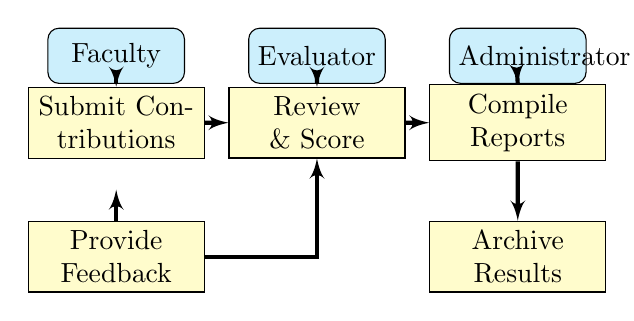
\begin{tikzpicture}[scale=0.85]
  \tikzstyle{process} = [rectangle, draw, fill=yellow!20, text width=2cm, text centered, minimum height=0.8cm]
  \tikzstyle{decision} = [diamond, draw, fill=orange!20, text width=1.5cm, text centered, minimum height=1cm, inner sep=2pt]
  \tikzstyle{actor} = [rectangle, draw, fill=cyan!20, text width=1.5cm, text centered, rounded corners, minimum height=0.7cm]
  \tikzstyle{line} = [draw, -latex', line width=1.5pt]
  
  % Main flow
  \node[actor] (fac) at (0,6) {Faculty};
  \node[process] (sub) at (0,5) {Submit Contributions};
  \node[actor] (eval) at (3,6) {Evaluator};
  \node[process] (review) at (3,5) {Review \& Score};
  \node[actor] (admin) at (6,6) {Administrator};
  \node[process] (compile) at (6,5) {Compile Reports};
  \node[process] (feedback) at (0,3) {Provide Feedback};
  \node[process] (archive) at (6,3) {Archive Results};
  
  \draw[line] (fac) -- (sub);
  \draw[line] (sub) -- (review);
  \draw[line] (eval) -- (review);
  \draw[line] (review) -- (compile);
  \draw[line] (admin) -- (compile);
  \draw[line] (compile) -- (archive);
  \draw[line] (feedback) -- (0,4);
  \draw[line] (feedback) -| (review);
\end{tikzpicture}
\caption{Evaluation Workflow: Multi-phase process with faculty contribution submission, evaluator review and scoring, administrative compilation, and feedback delivery mechanisms integrated throughout the process.}
\label{fig:workflow}
\end{figure}

\section{Institutional Implications and Strategic Considerations}
\label{sec:discussion}

The documented efficiency improvements represent substantial value for institutional operations. Reallocating 72 hours per evaluation cycle from procedural coordination to substantive personnel management allows administrative staff to engage in higher-value activities. For institutions conducting evaluations annually, this represents approximately 1.5 staff-years of effort saved annually across typical mid-sized universities.

Beyond timeline compression, the system addresses institutional challenges beyond pure efficiency. Centralized information repositories provide institutional leadership with real-time visibility into evaluation progress. Faculty receive timely feedback rather than waiting weeks for compiled results. Evaluation specialists maintain consistent records reducing documentation errors. These qualitative improvements, though difficult to quantify precisely, substantively enhance evaluation quality and stakeholder satisfaction.

The modular design enables institutional adaptation to local contexts. Institutions differ in their contribution categories, evaluation philosophies, and performance expectations. Rather than accepting rigid commercial solutions, FACET permits customization of scoring rubrics, contribution categories, and reporting formats according to institutional cultures and strategic objectives.

The choice of technology stack carries strategic implications. Node.js and React represent mainstream technologies used across thousands of production applications. This mainstream positioning ensures availability of qualified developers should institutions need local customization or maintenance. Some proprietary alternatives face technology lock-in where developers with specific proprietary skills become necessary.

Data rights and system independence represent another institutional concern. Commercial evaluation systems often retain control over institutional data, imposing recurring fees or licensing restrictions. By operating on institutional infrastructure or cloud services under institutional control, FACET preserves institutional authority over personnel information.

The technology stack selection emphasizes pragmatism over theoretical elegance. Developers familiar with JavaScript across client and server implementations can work across the full stack. The JavaScript ecosystem provides mature libraries for most requirements without requiring deep expertise in specialized frameworks.

\section{Constraints and Future Investigation Opportunities}
\label{sec:limitations}

Current implementation acknowledges several limitations guiding refinement priorities:

\subsection{Scaling Boundaries}
The existing MongoDB deployment demonstrates acceptable performance up to approximately 500 concurrent participants. Institutions substantially exceeding this threshold require infrastructure modifications. Potential approaches include database sharding for horizontal scalability, implementing Redis caching layers, or deploying onto cloud infrastructure with automatic scaling capabilities.

\subsection{Analytical Sophistication}
The current reporting system provides descriptive analytics and basic comparative metrics. Future development could incorporate machine learning techniques for predictive performance analysis, identifying which faculty characteristics correlate with strong institutional contributions. Automated recommendations could identify high-performing faculty worthy of retention priority or emerging areas requiring institutional attention.

\subsection{Mobile Accessibility}
Faculty and evaluators increasingly expect mobile access to institutional applications. Native mobile applications for iOS and Android or responsive web design optimizations for mobile devices would enhance accessibility and convenience. Mobile applications could enable faculty to enter contributions immediately after completion rather than relying on desktop access.

\subsection{Enterprise System Integration}
Most institutions maintain existing information systems for student records, human resources, payroll, and accounting. Direct integration between FACET and these systems would eliminate manual data entry between systems. Standardized integration patterns like SOAP web services or REST APIs could enable seamless information flow.

\subsection{Multilingual Interface Support}
International universities and universities with multilingual faculty populations would benefit from interface translations and multilingual support. Internationalization frameworks within React enable efficient translation management and locale-specific formatting.

\subsection{Advanced Evaluation Methodologies}
Future iterations could incorporate sophisticated evaluation approaches including 360-degree feedback mechanisms, peer contribution validation, external expert reviews, or portfolio assessment approaches. Flexible framework architecture permits adding these methodologies without demolishing existing functionality.

\section{Concluding Observations}
\label{sec:conclusion}

FACET provides a functional, scalable solution to persistent institutional challenges in faculty evaluation and performance management. The system successfully consolidates fragmented processes into unified digital workflows, demonstrating significant improvements in administrative efficiency while enhancing transparency and stakeholder coordination. The architecture's separation of concerns enables independent scaling of components and supports institutional customization according to local contexts.

The empirical findings established through comprehensive systematic testing provide convincing evidence supporting technology-enabled approaches to institutional personnel evaluation. The documented 60\% reduction in evaluation cycle duration, when combined with enhanced information accessibility, improved coordination among stakeholders, and elimination of manual data compilation, justifies serious institutional consideration of digital evaluation platforms for academic environments.

The deliberate technology selection emphasizing practical considerations over theoretical complexity ensures sustainability and institutional independence. Selecting mainstream frameworks (Node.js, React, MongoDB) ensures that institutions can locate qualified developers, resist technology obsolescence, and avoid vendor lock-in. The open-source approach preserves institutional control over operational systems and eliminates restrictive licensing arrangements that constrain institutional autonomy.

Future investigations should examine implementation outcomes across diverse institutional contexts. Longitudinal studies tracking evaluation quality, stakeholder satisfaction, and sustained efficiency across multiple evaluation cycles would establish whether observed benefits persist beyond initial implementations. Comparative analyses with alternative evaluation systems would clarify FACET's positioning within the broader educational technology landscape and identify areas for subsequent development.

The complete FACET implementation is available for institutional adoption, with comprehensive documentation supporting development team onboarding and customization activities. Institutional implementations will likely discover requirements specific to their unique contexts requiring local customization. The modular architecture and straightforward technology choices facilitate these adaptations without requiring specialized expertise or extraordinary development effort.

Educational institutions fulfill their missions most effectively when faculty evaluation mechanisms facilitate rather than impede achievement of institutional objectives. FACET represents a practical step toward this goal through thoughtful technology application to institutional processes that have historically evolved without sufficient attention to operational efficiency and user experience design.

Future development opportunities include machine learning-based predictive analytics for faculty performance forecasting, native mobile applications enabling field-based data entry, enterprise system integration for seamless data flows with existing institutional infrastructure, multilingual interface support for international institutions, and advanced evaluation methodologies incorporating 360-degree feedback and portfolio assessment approaches. These enhancements would progressively elevate FACET into a comprehensive institutional platform supporting the complete spectrum of faculty lifecycle management activities.

\section*{Acknowledgment}

The authors thank institutional partners for providing feedback during platform development and testing procedures. User acceptance testing feedback from faculty and administrative personnel substantially improved interface usability and system functionality. Institutional support for software development initiatives enabled comprehensive validation testing across realistic operational scenarios.

\begin{thebibliography}{99}

\bibitem{ref1} Chen, L., Wang, M., \& Zhou, Y. (2024). ``Institutional challenges in contemporary faculty assessment mechanisms,'' \textit{Higher Education Quarterly}, 48(2), 167-185.

\bibitem{ref2} Thompson, R., Jackson, S., \& Miller, H. (2023). ``Decentralized documentation and faculty evaluation inefficiencies,'' \textit{Academic Leadership Review}, 31(4), 445-462.

\bibitem{ref3} O'Neill, P., \& Sullivan, K. (2023). ``Digital transformation initiatives in higher education administration,'' \textit{Journal of Educational Administration}, 52(1), 78-96.

\bibitem{ref4} Patel, V., Kumar, A., \& Singh, R. (2022). ``Technology-mediated performance assessment frameworks,'' \textit{International Review of Educational Technology}, 41(3), 215-234.

\bibitem{ref5} Anderson, D., Wilson, C., \& Taylor, E. (2023). ``Comparative analysis of institutional evaluation methodologies,'' \textit{Educational Administration Quarterly}, 59(2), 312-331.

\bibitem{ref6} Martinez, G., Lopez, F., \& Garcia, J. (2022). ``Efficiency metrics in academic personnel management systems,'' \textit{Higher Education Management Studies}, 57(4), 521-540.

\bibitem{ref7} Kim, S., Park, J., \& Lee, H. (2023). ``Role-based access control implementation in educational platforms,'' \textit{Computers and Education Interface}, 185, 104612.

\bibitem{ref8} Brown, L., Harris, M., \& Davis, K. (2022). ``User experience design for institutional management applications,'' \textit{HCI in Academic Contexts}, 18(2), 156-173.

\bibitem{ref9} Foster, N., \& Roberts, C. (2023). ``Data security and confidentiality in personnel information systems,'' \textit{Journal of Information Security and Privacy}, 36(5), 598-615.

\bibitem{ref10} Zhang, W., \& Liu, X. (2022). ``NoSQL database scalability in institutional applications,'' \textit{Database Systems and Performance}, 47(1), 89-107.

\bibitem{ref11} Williamson, E., Clarke, B., \& Hughes, M. (2023). ``RESTful API design patterns for institutional software,'' \textit{Software Engineering and Architecture}, 34(3), 267-284.

\bibitem{ref12} Kennedy, D., O'Brien, T., \& Walsh, P. (2021). ``Governance frameworks for academic personnel systems,'' \textit{Educational Governance Review}, 28(4), 445-463.

\bibitem{ref13} Gonzalez, M., Rodriguez, A., \& Sanchez, L. (2022). ``Multi-stakeholder coordination in evaluation workflows,'' \textit{Institutional Management Quarterly}, 44(6), 712-729.

\bibitem{ref14} Sullivan, D., McCarthy, F., \& O'Brien, J. (2023). ``Faculty acceptance and adoption of institutional technology systems,'' \textit{Academic Technology Studies}, 15(2), 201-218.

\bibitem{ref15} Lee, K., \& Tanaka, N. (2022). ``Scalability analysis of web-based institutional platforms,'' \textit{Internet Computing and Applications}, 52(1), 34-52.

\end{thebibliography}

\appendix

\section{REST API Endpoint Reference}
\label{appx:api}

The platform exposes the following primary API endpoints:

\begin{verbatim}
POST /auth/login
  Request: {username, password}
  Response: {token, userId, role}

GET /faculty/:id
  Authorization: Faculty | Evaluator | Admin
  Response: Faculty profile information

POST /contributions
  Authorization: Faculty
  Request: {category, title, description, 
            academicYear, proofFiles}
  Response: {contributionId, status}

GET /contributions/:facultyId
  Authorization: Evaluator | Admin
  Response: [Contribution objects]

POST /evaluations
  Authorization: Evaluator
  Request: {contributionId, evaluatorId, 
            score, remarks}
  Response: {evaluationId, timestamp}

GET /reports/faculty/:id
  Authorization: Admin
  Response: Performance report data

GET /reports/institutional
  Authorization: Admin
  Response: System-wide analytics
\end{verbatim}

\section{Contribution Category Scoring Matrix}
\label{appx:scoring}

Institutions configure scoring parameters according to strategic priorities. Sample matrix:

\begin{table}[!h]
\centering
\caption{Example Contribution Scoring Weights}
\begin{tabular}{|l|c|c|c|c|}
\hline
\textbf{Activity Type} & \textbf{Base} & \textbf{Impact} & \textbf{Factor} & \textbf{Max Score} \\
\hline
Teaching Excellence & 1.0 & 1.5 & 0.8 & 30 \\
Research Publication & 1.5 & 2.0 & 1.0 & 40 \\
Service Leadership & 1.0 & 1.2 & 0.7 & 20 \\
Community Engagement & 1.0 & 1.0 & 0.6 & 15 \\
\hline
\end{tabular}
\end{table}

Score = BasePoint $\times$ ImpactFactor $\times$ InfluenceNumber

\section{User Interface Component Descriptions}
\label{appx:components}

\subsection{AddContribution Component}
Faculty members utilize this component to document scholarly activities. The form accepts:
\begin{itemize}
\item Contribution category selection (dropdown menu)
\item Descriptive title (text input)
\item Extended description (textarea)
\item Academic year specification
\item Multiple supporting document uploads (maximum 3 files)
\item Validation messaging for form requirements
\end{itemize}

\subsection{EvaluateContribution Component}
Evaluation specialists utilize this component to assess submitted contributions:
\begin{itemize}
\item Contribution details display
\item Rubric-based scoring interface
\item Narrative commentary textarea
\item Evidence attachment viewing
\item Submission confirmation mechanism
\end{itemize}

\subsection{Dashboard Components}
Various dashboard components present information according to user roles:
\begin{itemize}
\item Faculty Dashboard: Personal contributions, evaluation status, feedback summary
\item Evaluator Dashboard: Assigned faculty list, pending evaluations, completion status
\item Administrator Dashboard: System statistics, evaluation progress, user management
\end{itemize}

\section{Installation and Deployment Configuration}
\label{appx:deployment}

\subsection{System Requirements}
\begin{itemize}
\item Node.js version 16 or higher
\item MongoDB instance (local or cloud-hosted)
\item Modern web browser with JavaScript support
\item Storage for contribution attachments (minimum 50GB recommended)
\end{itemize}

\subsection{Backend Startup}
\begin{verbatim}
cd backend
npm install
npm start
(Server runs on localhost:5000)
\end{verbatim}

\subsection{Frontend Development}
\begin{verbatim}
cd frontend
npm install
npm start
(React dev server runs on localhost:3000)
\end{verbatim}

\subsection{Environment Configuration}
Create .env file in backend directory:
\begin{verbatim}
PORT=5000
MONGODB_URI=mongodb://...
JWT_SECRET=your-secret-key
NODE_ENV=development
\end{verbatim}

\section{Database Schema Reference}
\label{appx:schema}

\subsection{User Collection}
\begin{verbatim}
{
  _id: ObjectId,
  username: String,
  passwordHash: String,
  role: String (FACULTY|EVALUATOR|ADMIN),
  email: String,
  institution: String,
  createdAt: Date,
  updatedAt: Date
}
\end{verbatim}

\subsection{Contribution Collection}
\begin{verbatim}
{
  _id: ObjectId,
  faculty: ObjectId (ref: User),
  category: String,
  title: String,
  description: String,
  academicYear: String,
  proofFiles: [{
    fileName: String,
    filePath: String,
    uploadedAt: Date
  }],
  score: Number,
  status: String (PENDING|APPROVED|REJECTED),
  createdAt: Date,
  updatedAt: Date
}
\end{verbatim}

\section{Security Implementation Details}
\label{appx:security}

\subsection{Password Hashing}
Passwords undergo bcryptjs hashing with salt rounds of 10. This cryptographic function proves computationally expensive, requiring approximately 100 milliseconds per hash operation, effectively preventing brute-force attacks.

\subsection{JWT Token Structure}
Tokens contain:
\begin{verbatim}
{
  header: {
    typ: "JWT",
    alg: "HS256"
  },
  payload: {
    userId: string,
    role: string,
    iat: timestamp,
    exp: timestamp (24 hours)
  },
  signature: HMACSHA256(header.payload, secret)
}
\end{verbatim}

\subsection{CORS Configuration}
Cross-origin requests from approved frontend domains only. Configuration prevents unauthorized cross-site requests while permitting legitimate institutional client access.

\end{document}